\documentclass{article}
\usepackage[pdftex]{graphicx} 
\usepackage{listings}
\usepackage{color}
\usepackage{multicol}
\usepackage{float}
\usepackage[margin=3.5cm]{geometry}
\usepackage[font=small,labelfont=bf]{caption}

\definecolor{dkgreen}{rgb}{0,0.6,0}
\definecolor{gray}{rgb}{0.5,0.5,0.5}
\definecolor{mauve}{rgb}{0.58,0,0.82}

\lstset{frame=tb,
  language=Python,
  aboveskip=3mm,
  belowskip=3mm,
  showstringspaces=false,
  columns=flexible,
  basicstyle={\small\ttfamily},
  numbers=none,
  numberstyle=\tiny\color{gray},
  keywordstyle=\color{blue},
  commentstyle=\color{dkgreen},
  stringstyle=\color{mauve},
  breaklines=true,
  breakatwhitespace=true,
  tabsize=3
}


\begin{document}
	\title{Evolving a Collection of Strings to a Target Sequence using Genetic Programming}
	\author{Ramón Reszat}
	\maketitle
		\begin{multicols}{2}
		\section{Introduction}
		Genetic search sequentially evolves a randomly chosen distribution of strings until a subset of the remaining genotypes have converged to a desired goal state. As an example of the types of problems encountered in this field we adapt the infinite monkey theorem \cite{infinitemonkey} to random text output produced as a population of \(N_p\) strings, getting cross combined over a number of \(N_g\) discrete steps. Introducing a fitness measure for the strings allows the algorithm to choose from the \(N_p\) fixed-size sequences and eventually terminate with an approximate solution. Thus the element of evolutionary pressure becomes a driving force to compose the desired sequence.

		\section{Methods}
		Using genetic programming the task becomes an optimization problem on the sequences described by the formal grammar
		\(G=(N,\Sigma,P,S)\).
		\[\Sigma=\{a,b,c,...,x,y,z\}\]
		\[S\rightarrow\{c_i \epsilon \Sigma\}_{l}\]
		The corresponding criterion can be defined as the error between the words of the language generated by \(G\) and the target sequence. Their Hamming distance \cite[p.~8f.]{hammingdistance}, the number of positions at which they differ, provides a measure of similarity and ensures that a fitness score \(s\) can be assigned to each element of \(L(G)\). Please see appendix B.
		Assuming the hit probability per character of \(\Sigma\) remains \(p=1/\Sigma\) and \(l=10\) is the sequence length, 
		the fitness scores are binomially distributed over the initial population.
		\[ B(s;l,p)=p^s (1-p)^{l-s} \]
		To pick a crossover operation \cite{naturalcomputation} consider the longest common sequence \cite{longestcommonseq} between two arbitrary words of \(L(G)\).
		\begin{figure}[H]
			\center
			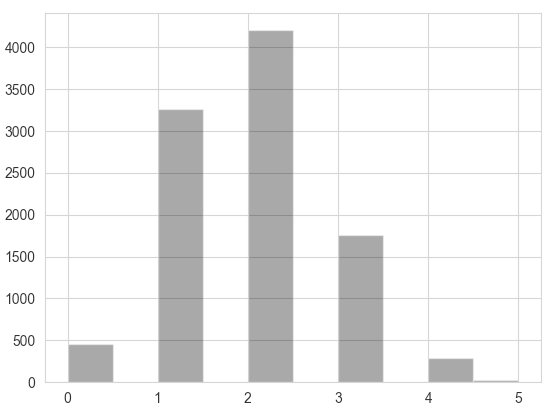
\includegraphics[width=\linewidth]{data/lcs_Np_10k.png}
			\caption{longest common sequence with goal state in \(N_p = 10000\)}
	  		\label{fig:lcs}
  		\end{figure}
  		We expect to find two consecutive letters in each word that match the target sequence (Figure \ref{fig:lcs}). In terms of the underlying grammar this means we can add a substructure to the production rules of G such that 
  		\[S\rightarrow\{A\}_{N}\]
  		\[A\rightarrow\{c_i\}_{l/N}\]
  		In this case the alignment of the resulting genes matters for matching to the target sequence.
  		Therefore we choose a random locus for the split und interchange at this position to produce two offsprings. This keeps the population size constant.
  		\begin{figure}[H]
			\center
			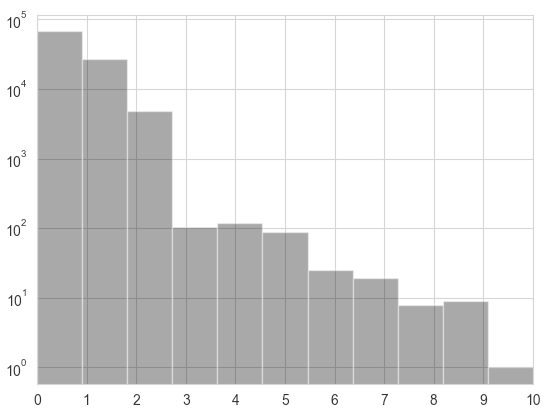
\includegraphics[width=\linewidth]{data/population_Ng20_k400.png}
			\caption{fitness distribution over \(N_p=100000\) at \(N_g=20\) (\(k=400, r=0.2\))}
	  		\label{fig:pop}
  		\end{figure}
  		For candidate selection we sort the population by fitness score and take the \(k\) best for cross combination.

  		Additionally mutation is introduced to switch a random position of the sequence to an arbitrary element of the alphabet \(\Sigma\). The chance of its occurance is denoted by the mutation rate \(r\).
  		{}
		\section{Results}{}
		The parameters \(k\) and \(r\) introduce diversity \cite{naturalcomputation} into the population at each iteration step by manipulating input and output of the elementary genetic operation. Choosing a sufficiently high \(k\) moves a bigger part of the population towards higher fitness scores (Figure \ref{fig:pop}). Please also refer to Figures 4-7 in appendix D.
		\begin{figure}[H]
			\center
			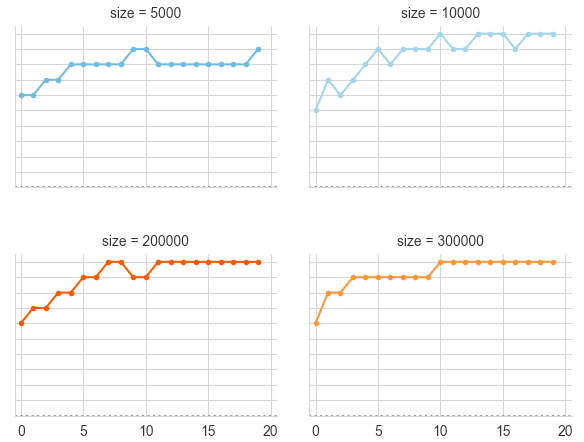
\includegraphics[width=\linewidth]{data/walk_Ng20_k400_snp_02.png}
			\caption{fitness score \(s\) after \(N_g\) steps with varying population size \(N_P\) (\(k=400, r=0.2\))}
	  		\label{fig:walk}
  		\end{figure}
  		Larger \(N_p\) results in the target sequence being more stable over a bigger number of steps (Figure \ref{fig:walk}).

  		Changing the mutation rate from \(r=0.1\) to \(r=0.3\) increases the probability to reach the target sequence faster within a smaller population \(N_p\). At the same time a higher mutation rate results into an instable best solution after further generations even for large \(N_p\). Compare Figures 8-11 in appendix E.
		\end{multicols}

		\bibliographystyle{unsrt}
		\bibliography{CNN_GA.bib}

		\newpage
		\appendix
		\section{Genetic Algorithm}
		\begin{lstlisting}
		def evolve(genotypes, select, mut_rate):
			selected_genotypes, suppressed_genotypes = select_k_best(genotypes, k=select)
			print(selected_genotypes[0])
			evolved_genotypes = crossover(selected_genotypes, locus=random.randrange(1,5))
			genotypes = evolved_genotypes + suppressed_genotypes
			genotypes = snp_mutation(genotypes, rate=mut_rate)
			return genotypes
		\end{lstlisting}
		\section{Fitness Function}
		\begin{lstlisting}
		def fitness_score(individual):
			# scale fitness between 0 and 10
			return len(individual) - hamming_distance(individual, target)
		\end{lstlisting}
		\begin{lstlisting}
		def hamming_distance(ind1, ind2):
			if len(ind1) == len(ind2):
				count = 0
				for i in range(len(ind1)):
					if ind1[i]!=ind2[i]:
						count+=1
				return count
		\end{lstlisting}
		\section{Crossover Function}
		\begin{lstlisting}
		def crossover(genotypes, locus=3, n_loci=5):
			children = []
			for i in range(int(len(genotypes)/2)):
				x = genotypes.pop()[1]
				y = genotypes.pop()[1]
				pos = locus * len(x)//n_loci
				children.append(x[:pos]+y[pos:])
				children.append(y[:pos]+x[pos:])
			return list(map(lambda ind: (fitness_score(ind), ind), children))
		\end{lstlisting}
		\newpage
		\section{K-best Selection}
		\begin{lstlisting}
		def select_k_best(genotypes, k):
			genotypes.sort(reverse=True, key=lambda ind: ind[0])
			selected = genotypes[:k]
			suppressed = genotypes[k:]
			return selected, suppressed
		\end{lstlisting}
		\begin{multicols}{2}
		\begin{figure}[H]
			\center
			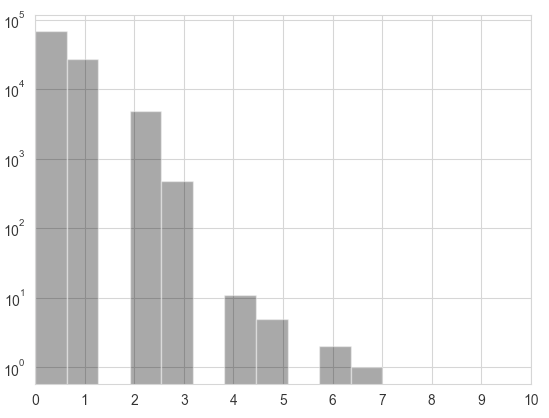
\includegraphics[width=\linewidth, height=120pt]{data/population_Ng20_k25.png}
			\caption{\(N_g=20, k=25, r=0.2\)}
	  		\label{fig:popNg20k25}
  		\end{figure}
  		\begin{figure}[H]
			\center
			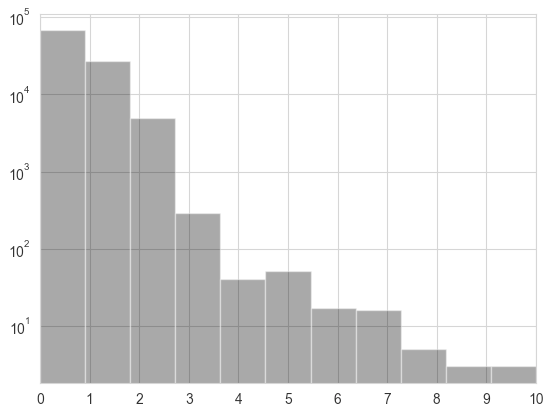
\includegraphics[width=\linewidth, height=120pt]{data/population_Ng20_k200.png}
			\caption{\(N_g=20, k=200, r=0.2\)}
	  		\label{fig:popNg20k200}
  		\end{figure}
  		\begin{figure}[H]
			\center
			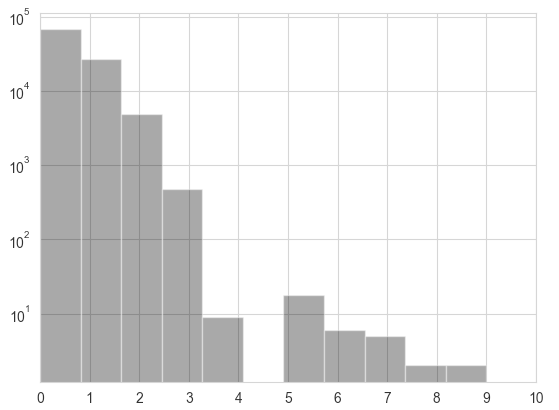
\includegraphics[width=\linewidth, height=120pt]{data/population_Ng20_k50.png}
			\caption{\(N_g=20, k=50, r=0.2\)}
	  		\label{fig:popNg20k50}
  		\end{figure}
  		\begin{figure}[H]
			\center
			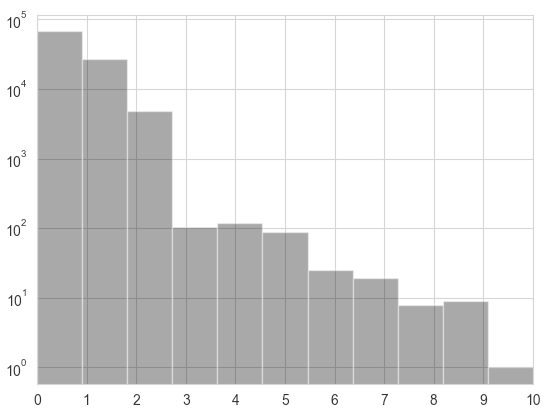
\includegraphics[width=\linewidth, height=120pt]{data/population_Ng20_k400.png}
			\caption{\(N_g=20, k=400, r=0.2\)}
	  		\label{fig:popNg20k400}
  		\end{figure}
  		\end{multicols}
		\newpage
		\section{SNP Mutation}
		\begin{lstlisting}
		def snp_mutation(genotypes, rate=0.2):
			for genotype in genotypes:
				if(random.random() < rate):
					genotype[1][random.randint(0,len(genotype[1])-1)] = random.choice(alphabet)
			return list(map(lambda ind: (fitness_score(ind[1]), ind[1]), genotypes))
		\end{lstlisting}
		\begin{multicols}{2}
		\begin{figure}[H]
			\center
			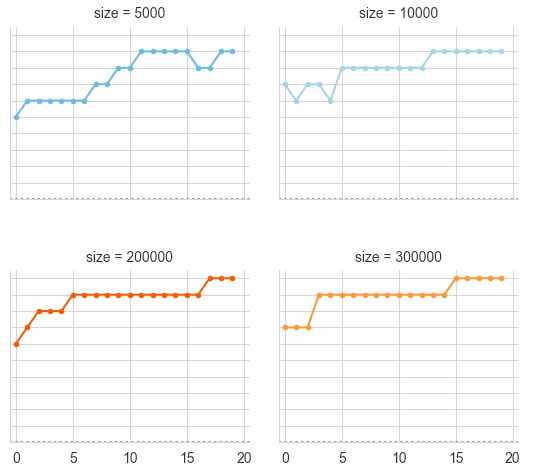
\includegraphics[width=\linewidth, height=120pt]{data/walk_Ng20_k200_snp_01.png}
			\caption{\(k=200, r=0.1\)}
	  		\label{fig:walk200ksnp01}
  		\end{figure}
  		\begin{figure}[H]
			\center
			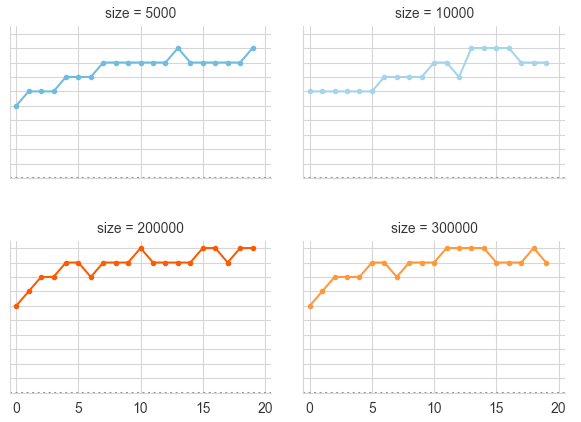
\includegraphics[width=\linewidth, height=120pt]{data/walk_Ng20_k200_snp_03.png}
			\caption{\(k=200, r=0.3\)}
	  		\label{fig:walk200ksnp03}
  		\end{figure}
  		\begin{figure}[H]
			\center
			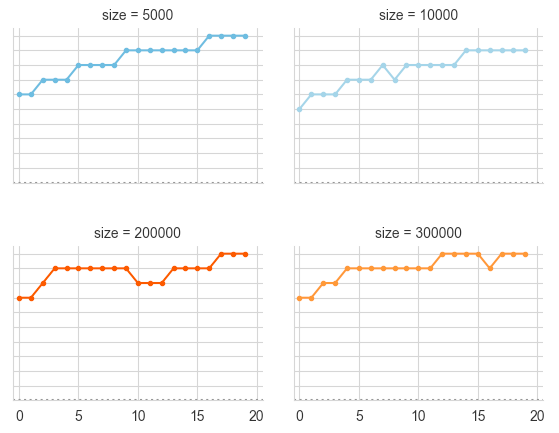
\includegraphics[width=\linewidth, height=120pt]{data/walk_Ng20_k200_snp_02.png}
			\caption{\(k=200, r=0.2\)}
	  		\label{fig:walk200ksnp02}
  		\end{figure}
  		\begin{figure}[H]
			\center
			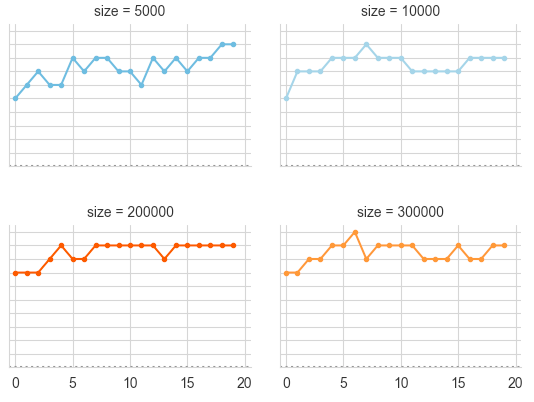
\includegraphics[width=\linewidth, height=120pt]{data/walk_Ng20_k200_snp_05.png}
			\caption{\(k=200, r=0.5\)}
	  		\label{fig:walk200ksnp05}
  		\end{figure}
  		\end{multicols}	
\end{document}